\documentclass[review]{elsarticle}


%% The amssymb package provides various useful mathematical symbols
\usepackage{amssymb}
\usepackage{natbib}
\usepackage{graphicx}
\usepackage{amsmath}
\usepackage{tabularx}
\usepackage{gensymb}
\usepackage[utopia]{mathdesign}
\usepackage[OMLmathrm,OMLmathbf,OMLmathsf,sfdefault=fav,scaled=0.875]{isomath}
\usepackage{color} % needed for the color change in TODO
\usepackage{gensymb} % needed for the degree C
%\usepackage{mathtools} 
\usepackage{caption}
\usepackage{subcaption}
\usepackage{epstopdf}
\usepackage{nomencl}
% \usepackage{german}
\usepackage{verbatim} 
\usepackage{xpatch}
\usepackage{framed} % Framing content
\usepackage{multicol} % Multiple columns environment
\makenomenclature%makeindex [].nlo -s nomencl.ist -o [].nls
\setlength{\nomlabelwidth}{.2\hsize}

\renewcommand{\nompreamble}{Throughout the article bold face symbols denote tensors and vectors. Normal face letters represent scalar quantities.}

\setlength{\nomitemsep}{-\parsep}

%Define groups for nomenclature

\RequirePackage{ifthen}

\renewcommand{\nomgroup}[1]{\bigskip%

\ifthenelse{\equal{#1}{R}}{\item[\textit{Roman symbols}]}{%

\ifthenelse{\equal{#1}{G}}{\item[\textit{Greek symbols}]}{\ifthenelse{\equal{#1}{O}}{\item[\textit{Operators}]}}}}


\newcommand{\tm}{\textrm}
\newcommand{\var}{\varepsilon}
\newcommand{\si}{\sigma}
\newcommand{\beq}{\begin{equation}}
\newcommand{\eeq}{\end{equation}}
\newcommand{\nn}{\nonumber}
\newcommand{\mwith}{\quad \mathrm{with} \quad}
\newcommand{\mand}{\quad \mathrm{and} \quad}
\newcommand{\mdiv}{\,\mathrm{div}\,}
\newcommand{\mDiv}{\,\mathrm{Div}\,}
\newcommand{\grad}{\,\mathrm{grad}\,}
\newcommand{\Grad}{\,\mathrm{Grad}\,}
\newcommand{\Cel}{\,$^\circ$C}
\newcommand{\dcdot}{\mbf{\,:\,}}
\newcommand{\tr}{\mathrm{tr}\,}
\newcommand{\mathd}{\mathrm{d}}
\newcommand{\mathD}{\mathrm{D}}
\newcommand{\mdiag}{\,\mathrm{diag\,}}
%\newcommand{\mbf}[1]{\mbox{${\mbox{\boldmath${#1}$\unboldmath}}$}}
\newcommand{\fourtens}[1]{\mbox{${\mbox{\boldmath$\mathcal{#1}$\unboldmath}}$}}
\newcommand{\mbf}[1]{{\mathbf{#1}}}%tensors/matrices
\newcommand{\mbfs}{\boldsymbol}
\newcommand{\dev}{\stackrel{def}{=}}
\newcommand{\tbf}{\textbf}
\newcommand{\tit}{\textit}
\newcommand{\mrm}{\mathrm}
%\newcommand{\citep}[1]{(\cite{#1})}
%\newcommand{\citet}{\cite}

\newcommand{\tf}{$\rightarrow\ $}
\newcommand{\ds}{\displaystyle}
\newcommand{\mtd}[2]{\frac{\mathd_{#1}{#2}}{\mathd t}} %material time derivative
\newcommand{\ptd}[1]{\frac{\partial {#1}}{\partial t}} %partial time derivative
\newcommand{\pd}[2]{\frac{\partial {#1}}{\partial {#2}}} %partial derivative
\newcommand{\vint}[1]{\int \limits_\Omega {#1} \mathd \Omega} %volume integral
\newcommand{\sint}[2]{\int \limits_{\partial \Omega_{#1}} {#2} \mathd \Gamma}
\newcommand{\uexp}[1]{$^{\mathrm{{#1}}}$}%superscript
\newcommand{\uind}[1]{$_{\mathrm{{#1}}}$}%subscript

%\newcommand{\mvec}[1]{\uline{{#1}}}%Vektoren
%\newcommand{\mmat}[1]{\uuline{{#1}}}%Matrizen

\newcommand{\mvec}[1]{\mathsfbfit{#1}}%Vektoren
\newcommand{\mmat}[1]{\mathsfbfit{#1}}%Matrizen


\newcommand{\drop}[1]{\red \cancelto{0}{\black #1} \black}

\newcommand{\centerpic}[3]{\hspace{#1\textwidth}\resizebox{#2\textwidth}{!}{\includegraphics{#3}}}

\newcommand{\squote}[2]{\begin{quote}{\huge{``}}{#1}{\huge{''}}\end{quote}\hfill Aus: {#2}}

\newcommand{\todo}[1]{\textcolor{red}{#1}}
\newcommand{\correction}[1]{\textcolor{blue}{#1}}

\newcommand{\comments}[1]{\textcolor{blue}{#1}}

\usepackage{lineno,hyperref}
\modulolinenumbers[5]

\journal{Water Resource Research}

%%%%%%%%%%%%%%%%%%%%%%%
%% Elsevier bibliography styles
%%%%%%%%%%%%%%%%%%%%%%%
%% To change the style, put a % in front of the second line of the current style and
%% remove the % from the second line of the style you would like to use.
%%%%%%%%%%%%%%%%%%%%%%%

%% Numbered
%\bibliographystyle{model1-num-names}

%% Numbered without titles
%\bibliographystyle{model1a-num-names}

%% Harvard
%\bibliographystyle{model2-names.bst}\biboptions{authoryear}

%% Vancouver numbered
%\usepackage{numcompress}\bibliographystyle{model3-num-names}

%% Vancouver name/year
%\usepackage{numcompress}\bibliographystyle{model4-names}\biboptions{authoryear}

%% APA style
%\bibliographystyle{model5-names}\biboptions{authoryear}

%% AMA style
%\usepackage{numcompress}\bibliographystyle{model6-num-names}

%% `Elsevier LaTeX' style
\bibliographystyle{elsarticle-num}
%%%%%%%%%%%%%%%%%%%%%%%

\begin{document}

\begin{frontmatter}

\title{Analytical analysis of timescales of seawater intrusion and retreat}
%\tnotetext[mytitlenote]{Fully documented templates are available in the elsarticle package on \href{http://www.ctan.org/tex-archive/macros/latex/contrib/elsarticle}{CTAN}.}

%% Group authors per affiliation:
\author[label1,label2]{Tianyuan Zheng}
\ead{tianyuan.zheng@ufz.de}
\author[label3]{Bo Guo\corref{cor1}}
\ead{boguo@princeton.edu}
\cortext[cor1]{Corresponding author. Civil and Environmental Engineering, Princeton University}
\address[label1]{Department of Environmental Informatics, Helmholtz Centre for Environmental Research - UFZ, Permoserstra{\ss}e 15, 04318 Leipzig, Germany}
\address[label2]{Applied Environmental Systems Analysis, Dresden University of Technology, Germany}
\address[label3]{Civil and Environmental Engineering, Princeton University, NJ, US, 08544}
%\fntext[1]{UFZ, Germany}
%\fntext[2]{Civil and Environmental Engineering, Princeton University, NJ, US, 08544}

%% or include affiliations in footnotes:
%\author[mymainaddress,mysecondaryaddress]{Elsevier Inc}
%\ead[url]{www.elsevier.com}

%\author[mysecondaryaddress]{Global Customer Service%\corref{mycorrespondingauthor}}
%\cortext[mycorrespondingauthor]{Corresponding author}
%\ead{support@elsevier.com}

%\address[mymainaddress]{1600 John F Kennedy Boulevard, Philadelphia}
%\address[mysecondaryaddress]{360 Park Avenue South, New York}

\begin{abstract}

\end{abstract}

\begin{keyword}
Seawater intrusion, Timescale, Analytical analysis
\end{keyword}

\end{frontmatter}

\linenumbers

\section{Introduction}

\section{Methodology}

\subsection{Conceptual model}

The conceptual model used in this study was a confined coastal aquifer with length L and thickness B which is shown is Fig. \ref{fig:seawater_intrusion}. The left boundary is coast and the right boundary is the inland aquifer. $h_\mbf{s}$ is the initial seawater level and $h_\mbf{f}$ is the initial inland freshwater head. The initial condition is regarded to be steady state. 
\begin{figure}
\centering
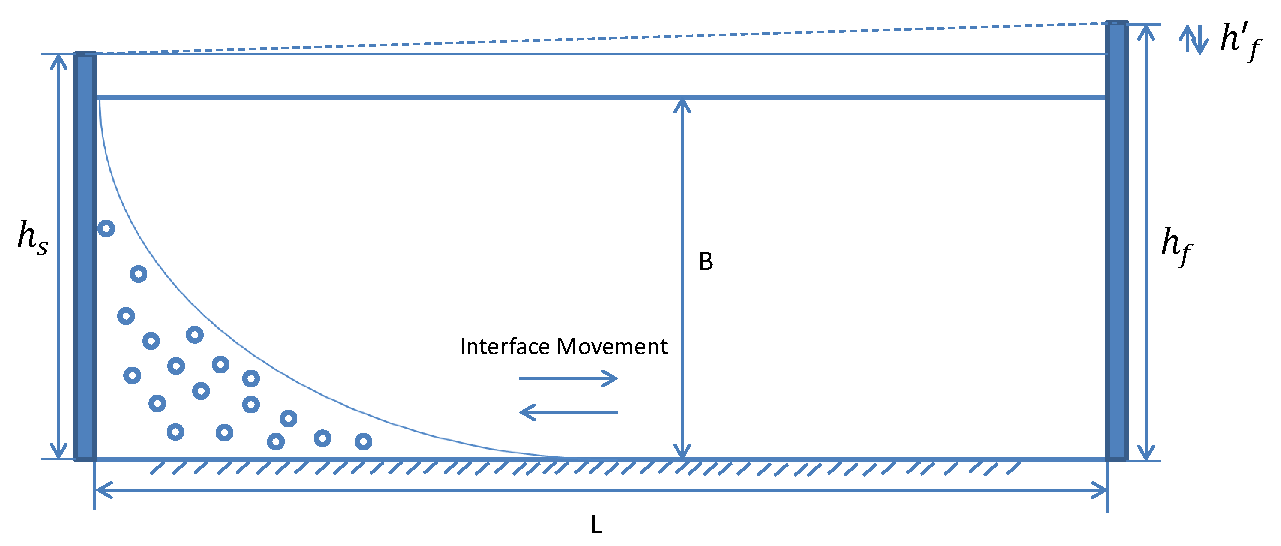
\includegraphics[width=1.0\textwidth]{figures/seawater_intrusion}
\caption{Conceptual model of the seawater intrusion and retreat. Following the same concept of \cite{lu2013timescales}}
\label{fig:seawater_intrusion}
\end{figure}

\subsection{Theoretical method}
Basic assumptions \cite{guo2002user}: 
\begin{itemize}
\item Darcy's flow is valid.  
\item The standard expression for specific storage in a confined aquifer is applicable.
\item The diffusive approach to dispersive transport is based on Fick's law.
\item Isothermal conditions prevails. 
\item The porous medium is fully saturated with water.
\item A single, fully miscible liquid phase of very small compressibility is taken in to account. 
\end{itemize}
%\he governing equations \cite{guo2002user}:
%conversions from native aquifer water and equivalent freshwater head is in Eq. \ref{eq:h_hf} and \ref{eq:hf_h}
%\begin{equation}\label{eq:h_hf}
%h_f = \frac{\rho}{\rho_f} - \frac{\rho - \rho_f}{\rho_f}Z 
%\end{equation}

%\begin{equation}\label{eq:hf_h}
%h = \frac{\rho_f}{\rho} + \frac{\rho - \rho_f}{\rho}Z 
%\end{equation}
%where $h_f$ is the equivalent freshwater head, $h$ is the native aquifer water head, $\rho$ is the density of saline ground water and $\rho_f$ is the density of fresh water.

%The governing equation for the conservation of mass is in \ref{eq:conservation_mass}
%\begin{equation}\label{eq:conservation_mass}
%-\nabla\cdot(\rho \mbf{q}) + \bar{\rho} q_\mbf{s} = \frac{\partial(\rho\theta)}{\partial t} 
%\end{equation}
%where $\mbf{q}$ is the specific discharge vector, $\bar{\rho}$ is the density of water entering from a source or leaving through a sink, $q_\mbf{s}$ is the volumetric flow rate per unit volume of aquifer representing sources and sinks, $\theta$ is porosity and $t$ is time. \par

%The left hand side of Eq. \ref{eq:conservation_mass} is the net flux of mass through the REV and the right hand side is the time rate of change in the mass stored in the REV which can be expanded with the chain rule: 
%\begin{equation}\label{eq:rho_theta_t}
%\frac{\partial \rho \theta}{\partial t} = \rho \frac{\partial \theta}{\partial t} + \theta\frac{\partial \rho}{\partial t} = \rho \frac{\partial \theta}{\partial P}\frac{\partial P}{\partial t} + \theta\frac{\partial \rho}{\partial P}\frac{\partial P}{\partial t} + \theta\frac{\partial \rho}{\partial C}\frac{\partial C}{\partial t}  
%\end{equation}
%where $C$ is the solute concentration and $P$ is the fluid pore pressure. 
The governing equations is based on \cite{ackerer1999modeling}. \\
The mass balance equation: 
\begin{equation}\label{eq:mass_conserv}
\rho S\frac{\partial P}{\partial t} + \phi \frac{\partial \rho}{\partial C_\mbf{m}}\frac{C_\mbf{m}}{\partial t} + \nabla\cdot(\rho\mbf{q}) = \rho Q_\mbf{s}
\end{equation}
where $S$ is the specific storativity of the porous medium, $\rho$ is the mass density of the fluid, $\mbf{q}$ is the Darcy velocity, $Q_\mbf{s}$ is the source/sink term, $\phi$ is the porosity and $C_\mbf{m}$ is the solute mass fraction. \\
The specific storativity $S$ is defined as:
\begin{equation}\label{eq:specific_S}
S = \alpha (1 - \phi) + \phi \beta
\end{equation} 
where $\alpha$ is the coefficient of compressibility of porous medium, $\beta$ is the coefficient of compressibility of the fluid:
\begin{equation}\label{eq:beta_alpha}
\beta = \frac{1}{\rho}\frac{\partial \rho}{\partial P}, \qquad \alpha = \frac{1}{1 - \phi}\frac{\partial \phi}{\partial P}
\end{equation}
The specific discharge is defined by the generalized Darcy's law:
\begin{equation}\label{eq:darcy_velocity}
\mbf{q} = - \frac{1}{\mu}\mbf{k}\cdot(\nabla P + \rho g \nabla z)
\end{equation}
where $\mu$ is the dynamic viscosity of the fluid, $\mbf{k}$ is the permeability tensor and $g$ is the gravity acceleration. \\
The solute transport equation:
\begin{equation}
\phi \rho \frac{\partial C_\mbf{m}}{\partial t} + \rho \mbf{q}\cdot\nabla C_\mbf{m} = \nabla\cdot(\phi \rho \mbf{D}\cdot\nabla C_\mbf{m})
\end{equation}
In which $\mbf{D}$ is the dispersion tensor. 









 

\section{Result and discussion}


\section*{References}

\bibliography{mybibfile}

\end{document}